\mychapter{11}{Lesson 11} %181031

% "The age of ULTRON" - wanted to keep that somewhere...
\section{Authenticated encryption (continued)}

Having proven that an authenticated encryption scheme in an \emph{Encrypt-then-Tag} mode is \cpa-secure, it remains to prove that it has the \textsc{auth} property. Before this, a new unforgeability definition is needed:

\begin{definition}
    Let $\Pi = (\textit{Tag}, \textit{Verify})$ be a \mac{} scheme. Then $\Pi$ is \textsc{eufcma}-secure iff it is \ufcma-secure, that is:
    \[
        \Pr[\cryptog{ufcma}(\lambda) = 1] \in \negl{\lambda}
    \]
    with the additional restriction that the tag $\phi^*$ of the forged message must be ``fresh'' itself.
\end{definition}

Note the small difference in security between \ufcma{} and \textsc{eufcma}.

\begin{theorem}
    Let $\Pi = (Enc, Dec, Tag, Verify)$ be an authenticated encryption scheme, composed by a \ske{} scheme $\Pi_1$ and a \mac{} scheme $\Pi_2$. If $\Pi_2$ is \textsc{eufcma}, then $\Pi$ has the \textsc{auth} property.
\end{theorem}

% AP190114: Need to phrase theorems differently
\begin{proof}
    The proof is analogous to the previous proof regarding the scheme's \cpa{} security. Suppose that $\Pi$ has not the \textsc{auth} property; then an adversary can use the distinguisher $\distinguisher^{\textsc{auth}}$ to successfully forge authenticated messages with fresh signatures against $\Pi_2$, as depicted in figure \ref{cryptoredux:ettauth}.
    
    \begin{cryptoredux}
        {ettauth}
        {Breaking authenticity of $\Pi_2$}
        {eufcma$_2$}
        {auth}[1.7]

        \cseqbeginloop

        \return{}{$m$}{}
        \send{$c \pickUAR Enc(k_{1}, m)$}{$c$}{}
        \receive{$\phi \pickUAR Tag(k_{2}, c)$}{$\phi$}{}
        \invoke{}{$(c, \phi)$}{\shortstack[r]{
            $c \in C$ \\
            $\phi \in \Phi$
        }}

        \cseqendloop

        \cseqdelay

        \return{\shortstack[r]{
            $c^* \notin C$ \\
            $\phi^* \notin \Phi$
        }}{$(c^{*}, \phi^{*})$}{}
        \send{}{$(c^*, \phi^*)$}{\shortstack[l]{
            \textsc{Output 1 iff} \\
            $\quad \textit{Verify}_k(c^*, \phi^*) = 1$}}

    \end{cryptoredux}

From $A^{auth}$ perspective, all the couples $(c_{i}, \phi_{i})$ received are made with the following schema:

\begin{equation*}
    c_{i} \in Enc(k_{1}, m \in \M) \wedge \phi_{i}\pickUAR Enc(k_{2}, c_{i})
\end{equation*}

Since $\A^{auth}$ wins $Game^{auth}$, the challenge couple $(c^{}{*}, \phi^{*})$ which breaks $Game^{auth}$ will be produced to be decrypted as

\begin{equation*}
    Dec(k, (c^{*}, \phi^{*})) \rightarrow Dec(k_{1}, c^{*}) \in \M \wedge
    Dec(k_{2}, \phi^{*})=c^{*}
\end{equation*}

But if this happens , then $\A$ can use the same challenge couple of $\A^{auth}$ to win $Game^{ufcma}$, which is impossible.

It could happen that, for $c^{*}=c$ previously seen, $\phi^{*}$ is a new fresh tag, never seen before. Just in this case the $auth$ game would be valid because $(c^{*}, \phi^{*})$ would have never been seen before, but \textbf{not } the eufcma game, because $c^{*}$ was previously sent to the challenger.
\end{proof}
    
Now we want an ufcma secure scheme able to resist against message-tag challenge couples where the tag is fresh but the message has been already requested to the challenger.

\section{Pseudorandom permutations}

\todo{Luby-Rackoff is cited here, but it's related to both \prf{}s-\prp{}s and the Feistel network analysis} 

Nothing prevents a \prf{} $F_k$ to be bijective; in this case, it is referred to as a \emph{pseudorandom permutation}, or \prp{} in short. Their definition is analogous to a generic \prf: as shown in figures \ref{cryptogame:prpreal} and \ref{cryptogame:prpideal}, \prp{}s are computationally indistinguishable from a random permutation:
\[
    Real_{\F, \A}(\lambda) \approx_{c} Ideal_{\F, \A}(\lambda)
\]
An important difference is that $F_k$ is efficiently invertible, although knowledge of $k$ is reqiuired in order to do so.

\begin{cryptogame}
    {prpreal}
    {$Real_{\F, \A}(\lambda)$}
    {}

    \cseqchallenger{$k \pickUAR \binary^\lambda$}

    \cseqbeginloop
    \send{}{$x$}{}
    \receive{$y = F_k(x)$}{$y$}{}
    \cseqendloop

    \send{}{$b'$}{}
    
\end{cryptogame}

\begin{cryptogame}
    {prpideal}
    {$Ideal_{\P, \A}(\lambda)$}
    {}

    \cseqchallenger{$P \pickUAR \P(\lambda, n)$}

    \cseqbeginloop
    \send{}{$x$}{}
    \receive{$y = P(x)$}{$y$}{}
    \cseqendloop

    \send{}{$b'$}{}
    
\end{cryptogame}

\subsection{Feistel network}

\textsc{Prp}s have been successfully constructed by using existing \prf{}s into what is called a \emph{Feistel network}. As a starting point, let $F : \binary^n \to \binary^n$ be a \prf, and define the function $\psi_F$ as follows:

\begin{align*}
    \psi_F(x, y) &= (y, x \xor F(y)) = (x', y') \\
    \psi^{-1}_F(x', y') &= (F(x') \xor y', x') = (F(y) \xor x \xor F(y), y) = (x, y)
\end{align*}

\begin{figure}[ht]
    \centering
    
    \tikzstyle{box}  = [draw, minimum size=2em]

    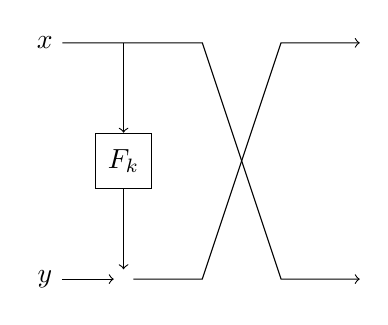
\begin{tikzpicture}[auto]
        
        \node (x) {$x$};
        \node (y) [below of = x, node distance = 3cm] {$y$};

        \node (xor) [right of = y] {$\xor$};
        \node (F) [box, above of = xor, node distance = 1.5cm] {$F_k$};

        \draw[->] (x) -- +(2cm, 0) -- +(3cm, -3cm) -- +(4cm, -3cm);
        \draw[->] (y) -- (xor);
        \draw[->] (xor) -- +(1cm, 0) -- +(2cm, 3cm) -- +(3cm, 3cm);

        \draw[->] (x)+(1cm, 0)  -- (F);
        \draw[->] (F) -- (xor);
        
    \end{tikzpicture}
    
    \label{fig:feistel}
    \caption{A single-round Feistel network}
\end{figure}

% AP190121: Some more intermediate steps might be useful
While this construct is invertible and uses a \prf{}, it is not pseudorandom itself, because the first $n$ bits of $\psi_{F}$'s image are always equal to $y$, and thus visible to any adversary. A first attempt at fixing this vulnerability would be to apply the construct two times on two different \prf{}s $\psi^2_{F, F'}$, in an attempt to ``hide'' $y$. Yet, this approach still leaks valuable information:
\[
    \psi_{F, F'}(x, z) \xor \psi_{F, F'}(y, z) = (x \xor y, \dots)
\]

However, this example with additional restrictions will be useful very soon, so it is reworded as the following lemma:

\begin{lemma}
    For any unbounded adversary making $q \in \poly(\lambda)$ queries, the following games in figure \ref{fig:feisteltwins} are statistically close as long as $y_1, \ldots, y_q$ are mutually distinct.
\end{lemma}

% AP190122: Prefer a single, b-oriented game, but for the sake of compliance to the original lessons the sequences are drawn with the old environment
% AP190902: Now they are sideways in the new environment, what did I mean back then?!
\begin{figure}[ht]
    \centering
    \begin{cryptogame}{}{}{}[0.5]
        \send{}{$x, y$}{}
        \receive{\small{$F, F' \pickUAR \R(\lambda, n, n)$}}{$\psi^2_{F, F'}(x, y)$}{}
    \end{cryptogame}
    \begin{cryptogame}{}{}{}[0.5]
        \send{}{$x, y$}{}
        \receive{\small{$R \pickUAR \R(\lambda, 2n, 2n)$}}{$R(x, y)$}{}
    \end{cryptogame}

    \caption{The two Feistel games}
    \label{fig:feisteltwins}
\end{figure}

\begin{proof}
    \todo{Idea: Hybridize over the queries before the challenge, from PR to random; prove that the stat distance between i and i+1 is negligible}
\end{proof}


Going back to the Feistel networks in general, it should be easy to see that they can be made of an arbitrary number of rounds, by simply chaining output with input. The $l$-th iteration is denoted as: 
\[
    \psi^l_\Phi(x, y) = \psi_{F}(\psi_{F''}( \ldots \psi_{F^{(l)}}(x, y) \ldots ))
\]
where $\Phi$ is the sequence of \prf{}s used at each single step. It can be shown that the rounds neeed to obtain a network that is indeed pseudorandom is just 3; also, the same \prf{} can be used, it is sufficient to change the seed on each iteration\footnotemark:

\begin{theorem}
    Let $F_i, F_j, F_k$ be a \prf{} over three seeds. Then $\psi^3_{i, j, k}$ is a \prp.
\end{theorem}

\footnotetext{That is actually the purpose of using a \prf}

\begin{proof}
    \todo{Idea: Four total games: original, swap prfs with random functions, swap the three functions with a single one (use previous lemma), swap random function with random permutation (avoid bad events generated by injection property)}
\end{proof}